\documentclass{article}
\usepackage{amsmath}
\usepackage{amssymb}
\usepackage{graphicx}
\usepackage{enumitem}
\usepackage{algorithm}
\usepackage{algpseudocode}
\usepackage{tcolorbox}
\usepackage{xcolor}
\usepackage{tikz}
\usepackage{hyperref}
\usepackage{geometry}

% Just narrower margins to save paper
\geometry{
  letterpaper,
  margin=0.75in
}

\DeclareMathOperator*{\argmax}{arg\,max}

\title{1. Reinforcement Learning: Sequential Decision Making}
\author{Notes based on Sutton \& Barto}


\begin{document}
% Add definitions for tikz libraries needed for diagrams
\usetikzlibrary{arrows.meta,shapes,positioning,shadows,trees,shapes.geometric,decorations.pathreplacing}

\maketitle
\tableofcontents
\newpage

\section{Index of Topics}
\begin{enumerate}[label=\arabic*.]
    \item \textbf{Sequential Decision Making}
    \begin{enumerate}[label=\arabic{enumi}.\arabic*.]
        \item Multi-armed Bandit Problem
        \item Actions, Rewards, and Policies
        \item Evaluative Feedback
        \item Incremental Update of Action-Values
        \item Exploitation vs. Exploration
        \item Action Sampling Methods
    \end{enumerate}
\end{enumerate}

\newpage

\section{Introduction to Sequential Decision Making}
Reinforcement learning is fundamentally about sequential decision making - the study of how agents learn to make a sequence of decisions that maximize cumulative reward over time. Unlike supervised learning where correct input-output pairs are presented, in reinforcement learning the agent must learn by interacting with its environment and discovering which actions yield the most reward.

The key challenge in sequential decision making is that decisions not only affect immediate rewards but may also influence future situations and, consequently, future rewards. This creates a temporal credit assignment problem: how do we attribute credit or blame to decisions that have delayed consequences?

\subsection{Multi-armed Bandit Problem}
The multi-armed bandit problem represents the simplest form of sequential decision making. The name comes from imagining a gambler at a row of slot machines (known as "one-armed bandits"), who must decide which machines to play, how many times to play each machine, and in which order to play them, to maximize reward.

This problem formulation is fundamental to reinforcement learning for several reasons:
\begin{itemize}
    \item It isolates the exploration-exploitation dilemma that is central to all reinforcement learning problems
    \item It provides a simplified setting with no state transitions, allowing us to focus solely on action selection
    \item It has important real-world applications such as clinical trials, website optimization, and adaptive routing
\end{itemize}

While simplified, the multi-armed bandit captures the essential challenge of learning from interaction: we must make decisions based on limited information, and our choices affect what information we receive in the future. This creates a feedback loop between learning and decision making.

\begin{figure}[h]
\centering
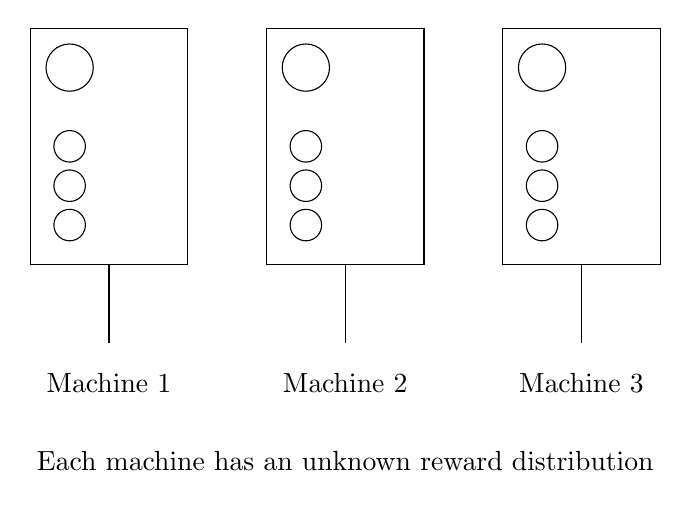
\begin{tikzpicture}
    % Draw slot machines
    \foreach \i in {1,2,3} {
        \draw (\i*3-3, 0) rectangle (\i*3-1, 3);
        \draw (\i*3-2.5, 2.5) circle (0.3);
        \draw (\i*3-2, 0) -- (\i*3-2, -1);
        \draw (\i*3-2.5, 1.5) circle (0.2);
        \draw (\i*3-2.5, 1) circle (0.2);
        \draw (\i*3-2.5, 0.5) circle (0.2);
    }
    % Labels
    \node at (1, -1.5) {Machine 1};
    \node at (4, -1.5) {Machine 2};
    \node at (7, -1.5) {Machine 3};
    \node at (4, -2.5) {Each machine has an unknown reward distribution};
\end{tikzpicture}
\caption{Illustration of a 3-armed bandit problem}
\end{figure}

\subsubsection{Problem Formulation}
In the multi-armed bandit problem:
\begin{itemize}
    \item You face $k$ different options or "arms"
    \item Each time step $t$, you select one arm $A_t \in \{1, 2, ..., k\}$
    \item After choosing arm $a$, you receive a reward $R_t$ drawn from a probability distribution associated with that arm
    \item The goal is to maximize the total reward $\sum_{t=1}^{T} R_t$ over some time horizon $T$
\end{itemize}

In mathematical terms, choosing an arm $a$ at time $t$ is formalized as an action from a set $\mathcal{A}$. When we choose action $A_t$, we receive a reward $R_t$ drawn from an unknown probability distribution $p(r|a)$.

\begin{equation}
    \text{Action selection:} \quad A_t \in \mathcal{A}
\end{equation}

\begin{tcolorbox}[colback=blue!5!white,colframe=blue!75!black,title=Notation Overview]
\begin{itemize}
    \item $A_t$: The action chosen at time $t$
    \item $\mathcal{A}$: The set of all possible actions
    \item $p(r|a)$: The probability distribution of reward $r$ given action $a$
    \item $R_t$: The reward received at time $t$ after taking action $A_{t-1}$ (following Sutton \& Barto's indexing)
\end{itemize}
\end{tcolorbox}

\subsection{Actions, Rewards, and Policies}
In the bandit problem, the agent's objective is to maximize the expected reward over time. The three fundamental components are:

\subsubsection{Actions}
Actions represent the choices available to the agent. In the multi-armed bandit setting, an action corresponds to selecting one of the $k$ arms. We denote the action taken at time $t$ as $A_t \in \mathcal{A}$, where $\mathcal{A}$ is the set of all possible actions.

\subsubsection{Rewards}
After taking action $A_t$ at time $t$, the agent receives a numerical reward $R_{t+1}$. This reward is sampled from a probability distribution associated with the selected action: $R_{t+1} \sim p(r|A_t)$. The distribution $p(r|a)$ is initially unknown to the agent and must be learned through experience.

\subsubsection{Policies}
A policy defines the agent's strategy for selecting actions. In the context of bandits, a policy $\pi$ is a mapping from actions to selection probabilities:

\begin{equation}
    \pi(a) = P(A_t = a)
\end{equation}

\begin{tcolorbox}[colback=blue!5!white,colframe=blue!75!black,title=Notation Overview]
\begin{itemize}
    \item $\pi(a)$: The probability of selecting action $a$ under policy $\pi$
    \item $P(A_t = a)$: The probability that the action at time $t$ equals $a$
\end{itemize}
\end{tcolorbox}

We can define more sophisticated policies that depend on past actions and rewards, but in the most basic form, a policy simply assigns probabilities to each action.

\subsection{Evaluative Feedback}
In reinforcement learning, the agent receives evaluative feedback rather than instructive feedback. The distinction is crucial:

\begin{itemize}
    \item \textbf{Instructive feedback} (as in supervised learning) tells the agent what the correct action would have been
    \item \textbf{Evaluative feedback} only indicates how good the selected action was, but not whether it was the best possible action or what the best action would have been
\end{itemize}

To understand the difference more clearly:
\begin{itemize}
    \item In supervised learning for image classification, if the model predicts "cat" when the true label is "dog", the model receives the correct label "dog" as feedback.
    \item In reinforcement learning, if an agent takes action $A_t$ and receives reward $R_{t+1}$, it only knows the value of that specific action—not what reward it would have received had it taken a different action or which action would have been optimal.
\end{itemize}

This approach mirrors many real-world learning scenarios. When a child touches a hot stove, they learn that this action led to pain, but they don't automatically know what alternative action would have been better. They must explore different approaches to build knowledge through experience.

Evaluative feedback forces the agent to actively explore to gather information about the environment, rather than passively receiving correct answers. This exploration process is what makes reinforcement learning fundamentally different from other machine learning paradigms.

The key challenge is to find the action $a$ that produces the maximum expected reward:

\begin{equation}
    \max_a \mathbb{E}[p(r|a)]
\end{equation}

\begin{tcolorbox}[colback=blue!5!white,colframe=blue!75!black,title=Notation Overview]
\begin{itemize}
    \item $\mathbb{E}[p(r|a)]$: The expected value of the reward distribution for action $a$
    \item $\max_a$: The operation of finding the action $a$ that maximizes the subsequent expression
\end{itemize}
\end{tcolorbox}

The true expected reward of each action is unknown, so the agent must estimate it from experience. This leads to the concept of action value.

\subsubsection{Action Value}
The value of an action $a$, denoted $q(a)$, is the expected reward when that action is selected:

\begin{equation}
    q(a) = \mathbb{E}[R_t | A_{t-1} = a]
\end{equation}

\begin{tcolorbox}[colback=blue!5!white,colframe=blue!75!black,title=Notation Overview]
\begin{itemize}
    \item $q(a)$: The true value of action $a$ (expected reward)
    \item $\mathbb{E}[R_t | A_{t-1} = a]$: The expected reward at time $t$ given that action $a$ was chosen at time $t-1$
\end{itemize}
\end{tcolorbox}

In practice, we estimate $q(a)$ based on observed rewards. Let $Q_t(a)$ denote our estimate of $q(a)$ at time $t$. As we gather more experience, we refine this estimate to approach the true value.

\begin{equation}
    Q_t(a) = \frac{1}{N_t(a)} \sum_{i=1}^{t} R_i \cdot \mathbf{1}_{A_{i-1}=a}
\end{equation}

\begin{tcolorbox}[colback=blue!5!white,colframe=blue!75!black,title=Notation Overview]
\begin{itemize}
    \item $Q_t(a)$: The estimated value of action $a$ at time $t$
    \item $N_t(a)$: The number of times action $a$ has been selected up to time $t$
    \item $R_i$: The reward received at time $i$
    \item $\mathbf{1}_{A_{i-1}=a}$: An indicator function that equals 1 if $A_{i-1} = a$ and 0 otherwise
\end{itemize}
\end{tcolorbox}

\subsection{Incremental Update of Action-Values}
Calculating $Q_t(a)$ using the formula above would require storing all past rewards, which becomes inefficient as $t$ grows. Instead, we can update our estimate incrementally after each new observation.

Incremental updating is a fundamental concept in reinforcement learning for several important reasons:

\begin{itemize}
    \item \textbf{Memory efficiency}: We don't need to store the entire history of rewards for each action
    \item \textbf{Computational efficiency}: We can update estimates with constant time complexity, regardless of how many steps we've taken so far
    \item \textbf{Online learning}: We can immediately incorporate new information as it becomes available
    \item \textbf{Non-stationarity}: With appropriate step sizes, we can track changing reward distributions over time
\end{itemize}

The incremental update approach is also aligned with how humans and animals appear to learn from experience. We don't reprocess our entire history of experiences when we learn something new; instead, we adjust our existing understanding based on new observations.

Let's derive the incremental update rule:

\begin{align}
    Q_{t+1}(a) &= \frac{1}{N_{t+1}(a)} \sum_{i=1}^{t+1} R_i \cdot \mathbf{1}_{A_{i-1}=a} \\
    &= \frac{1}{N_{t+1}(a)} \left( R_{t+1} \cdot \mathbf{1}_{A_{t}=a} + \sum_{i=1}^{t} R_i \cdot \mathbf{1}_{A_{i-1}=a} \right) \\
    &= \frac{1}{N_{t+1}(a)} \left( R_{t+1} \cdot \mathbf{1}_{A_{t}=a} + N_t(a) \cdot Q_t(a) \right)
\end{align}

If $A_{t} = a$, then $N_{t+1}(a) = N_t(a) + 1$ and the update becomes:

\begin{equation}
    Q_{t+1}(a) = Q_t(a) + \frac{1}{N_{t+1}(a)} [R_{t+1} - Q_t(a)]
\end{equation}

\begin{tcolorbox}[colback=blue!5!white,colframe=blue!75!black,title=Notation Overview]
\begin{itemize}
    \item $Q_{t+1}(a)$: The updated estimate of the value of action $a$ after observing the $(t+1)$-th reward
    \item $Q_t(a)$: The previous estimate of the value of action $a$
    \item $R_{t+1}$: The reward received at time $t+1$
    \item $\frac{1}{N_{t+1}(a)}$: The learning rate, which decreases as we observe more samples of action $a$
\end{itemize}
\end{tcolorbox}

This is known as the incremental update rule. It adjusts the current estimate $Q_t(a)$ by a fraction of the prediction error $[R_{t+1} - Q_t(a)]$. The prediction error represents the difference between the observed reward and the expected reward.

A more general form replaces $\frac{1}{N_{t+1}(a)}$ with a step-size parameter $\alpha \in (0,1]$:

\begin{equation}
    Q_{t+1}(a) = Q_t(a) + \alpha [R_{t+1} - Q_t(a)]
\end{equation}

\begin{tcolorbox}[colback=blue!5!white,colframe=blue!75!black,title=Notation Overview]
\begin{itemize}
    \item $\alpha$: The step-size parameter or learning rate, controlling how quickly the estimates are updated
    \item $[R_{t+1} - Q_t(a)]$: The prediction error or TD error
\end{itemize}
\end{tcolorbox}

Using a constant $\alpha$ can be advantageous in non-stationary problems where the true action values change over time. The constant step size gives more weight to recent rewards, allowing the estimates to track changing values.

\subsection{Exploitation vs. Exploration}
The multi-armed bandit problem presents a fundamental dilemma: exploitation versus exploration.

\begin{itemize}
    \item \textbf{Exploitation} means selecting the action that currently appears best based on accumulated knowledge
    \item \textbf{Exploration} means trying different actions to gather more information about their values
\end{itemize}

If we always exploit (by selecting the action with the highest estimated value), we risk missing better actions whose value we have underestimated due to limited samples. If we spend too much time exploring, we may waste opportunities to gain higher rewards from the best actions.

\begin{figure}[h]
\centering
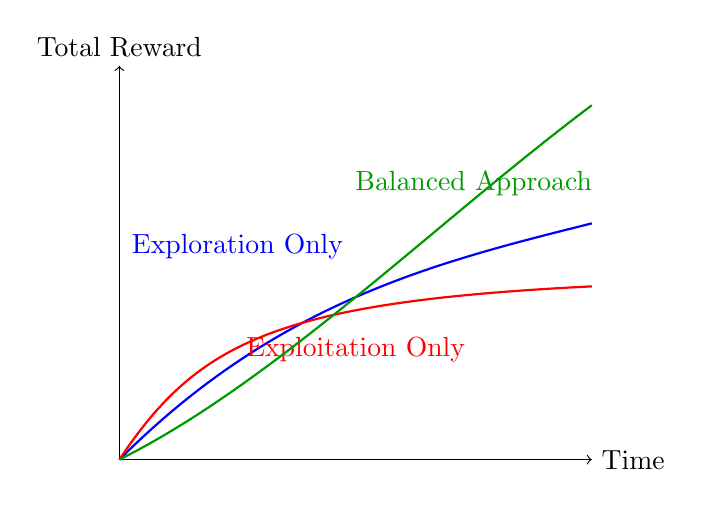
\begin{tikzpicture}
    % Axes
    \draw[->] (0,0) -- (6,0) node[right] {Time};
    \draw[->] (0,0) -- (0,5) node[above] {Total Reward};
    
    % Exploration only curve
    \draw[blue, thick] (0,0) .. controls (2,2) and (4,2.5) .. (6,3.0);
    \node[blue] at (1.5,2.7) {Exploration Only};
    
    % Exploitation only curve
    \draw[red, thick] (0,0) .. controls (1,1.5) and (2,2) .. (6,2.2);
    \node[red] at (3,1.4) {Exploitation Only};
    
    % Balanced approach curve
    \draw[green!60!black, thick] (0,0) .. controls (2,1) and (4,3) .. (6,4.5);
    \node[green!60!black] at (4.5,3.5) {Balanced Approach};
\end{tikzpicture}
\caption{Conceptual illustration of different exploration-exploitation strategies and their long-term reward outcomes}
\end{figure}

The exploration-exploitation dilemma extends far beyond reinforcement learning:

\begin{itemize}
    \item A restaurant-goer must decide whether to visit a new restaurant (exploration) or return to a favorite one (exploitation)
    \item A business must choose between investing in new products (exploration) or optimizing existing ones (exploitation)
    \item A researcher must decide whether to pursue novel research directions (exploration) or build on established findings (exploitation)
\end{itemize}

Finding the right balance is critical—too much exploitation leads to suboptimal solutions, while too much exploration wastes resources on unpromising options. Different contexts require different balances, and the optimal balance often changes over time as knowledge accumulates.

\subsubsection{Greedy Action Selection}
The simplest policy is to always select the action with the highest estimated value:

\begin{equation}
    A_t = \argmax_a Q_t(a)
\end{equation}

\begin{tcolorbox}[colback=blue!5!white,colframe=blue!75!black,title=Notation Overview]
\begin{itemize}
    \item $\argmax_a Q_t(a)$: The action $a$ that maximizes the estimated value $Q_t(a)$
\end{itemize}
\end{tcolorbox}

This policy is known as the greedy policy. It always exploits current knowledge but never explores, which can lead to suboptimal performance if the initial estimates are inaccurate.

\subsection{Action Sampling Methods}
Several methods have been developed to balance exploration and exploitation. Each has unique characteristics that make it suitable for different scenarios:

\subsubsection{$\epsilon$-Greedy Selection}
The $\epsilon$-greedy approach introduces random exploration by selecting a random action with probability $\epsilon$ and the greedy action with probability $1-\epsilon$:

\begin{equation}
    \pi(a) = 
    \begin{cases}
        1-\epsilon & \text{if } a = \argmax_a Q_t(a) \\
        \frac{\epsilon}{|\mathcal{A}|-1} & \text{otherwise}
    \end{cases}
\end{equation}

\begin{tcolorbox}[colback=blue!5!white,colframe=blue!75!black,title=Notation Overview]
\begin{itemize}
    \item $\pi(a)$: Probability of selecting action $a$
    \item $\epsilon$: The exploration rate $(0 \leq \epsilon \leq 1)$
    \item $|\mathcal{A}|$: The number of actions (cardinality of the action set)
    \item $\argmax_a Q_t(a)$: The action with the highest estimated value
\end{itemize}
\end{tcolorbox}

The $\epsilon$-greedy approach ensures that every action has some probability of being selected, which allows the agent to continue learning about all actions.

\textbf{Advantages of $\epsilon$-greedy:}
\begin{itemize}
    \item Simple to implement and understand
    \item Computationally efficient
    \item Guaranteed to eventually visit all actions
    \item Can be effective in practice despite its simplicity
\end{itemize}

\textbf{Implementation considerations:}
\begin{itemize}
    \item A common practice is to start with a high value of $\epsilon$ (e.g., 0.1) and gradually decrease it over time
    \item This approach, called \textit{$\epsilon$-decay}, allows more exploration early in learning when uncertainty is high
    \item As more information is gathered, $\epsilon$ decreases to favor exploitation
\end{itemize}

\begin{algorithm}
\caption{$\epsilon$-Greedy Action Selection}
\begin{algorithmic}[1]
\Procedure{EpsilonGreedy}{$Q_t, \epsilon$}
    \State $p \gets$ Random(0, 1)
    \If{$p < \epsilon$}
        \State \Return Random action from $\mathcal{A}$
    \Else
        \State \Return $\argmax_a Q_t(a)$
    \EndIf
\EndProcedure
\end{algorithmic}
\end{algorithm}

\subsubsection{Softmax Selection}
While $\epsilon$-greedy treats all non-greedy actions equally, the softmax approach (also known as Boltzmann exploration) selects actions with probabilities relative to their estimated values:

\begin{equation}
    \pi(a) = \frac{e^{Q_t(a)/\tau}}{\sum_{a' \in \mathcal{A}} e^{Q_t(a')/\tau}}
\end{equation}

\begin{tcolorbox}[colback=blue!5!white,colframe=blue!75!black,title=Notation Overview]
\begin{itemize}
    \item $\pi(a)$: Probability of selecting action $a$
    \item $e^{Q_t(a)/\tau}$: The exponential of the estimated value divided by temperature
    \item $\tau$: The temperature parameter controlling the randomness of the selection
    \item $\sum_{a' \in \mathcal{A}} e^{Q_t(a')/\tau}$: Normalization term to ensure probabilities sum to 1
\end{itemize}
\end{tcolorbox}

The temperature parameter $\tau$ controls the degree of exploration:
\begin{itemize}
    \item As $\tau \rightarrow 0$, softmax approaches greedy selection
    \item As $\tau \rightarrow \infty$, softmax approaches uniform random selection
\end{itemize}

\subsubsection{Upper Confidence Bound (UCB) Selection}
The UCB algorithm addresses the exploration-exploitation dilemma by selecting actions based not only on their estimated values but also on the uncertainty in those estimates:

\begin{equation}
    A_t = \argmax_a \left[ Q_t(a) + c \sqrt{\frac{\ln t}{N_t(a)}} \right]
\end{equation}

\begin{tcolorbox}[colback=blue!5!white,colframe=blue!75!black,title=Notation Overview]
\begin{itemize}
    \item $Q_t(a)$: The estimated value of action $a$ at time $t$
    \item $c$: A parameter controlling the degree of exploration
    \item $\ln t$: Natural logarithm of the current time step
    \item $N_t(a)$: The number of times action $a$ has been selected up to time $t$
    \item $\sqrt{\frac{\ln t}{N_t(a)}}$: The uncertainty term, which increases with time and decreases with the number of selections
\end{itemize}
\end{tcolorbox}

The UCB approach favors actions that either have high estimated values or have been selected infrequently. As an action is selected more often, its uncertainty term decreases, reducing the incentive for further exploration unless its estimated value is truly high.

\begin{figure}[h]
\centering
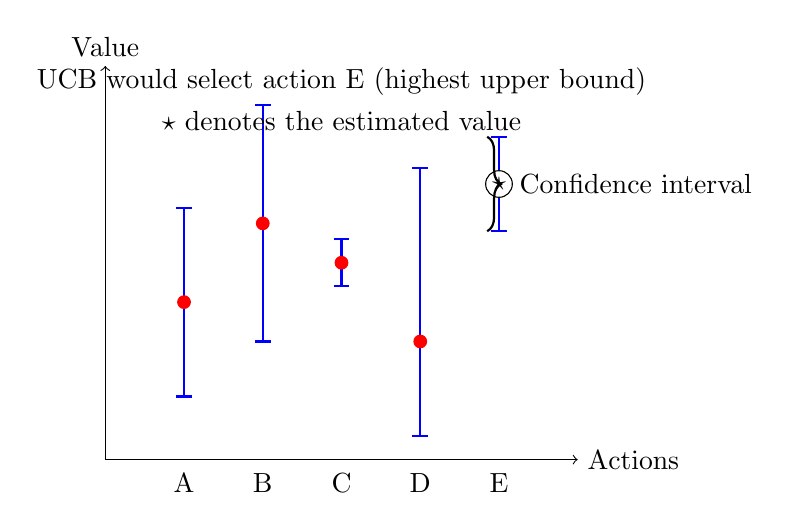
\begin{tikzpicture}
    % Draw confidence bounds
    \draw[->] (0,0) -- (6,0) node[right] {Actions};
    \draw[->] (0,0) -- (0,5) node[above] {Value};
    
    % Action values with confidence bounds
    \foreach \x/\y/\u/\l/\n in {1/2.0/3.2/0.8/A, 2/3.0/4.5/1.5/B, 3/2.5/2.8/2.2/C, 4/1.5/3.7/0.3/D, 5/3.5/4.1/2.9/E} {
        % Confidence bounds
        \draw[blue,thick] (\x,\l) -- (\x,\u);
        % Small horizontal lines at ends
        \draw[blue,thick] (\x-0.1,\l) -- (\x+0.1,\l);
        \draw[blue,thick] (\x-0.1,\u) -- (\x+0.1,\u);
        % Estimated value
        \filldraw[red] (\x,\y) circle (0.08);
        % Label
        \node at (\x,-0.3) {\n};
    }
    
    \node at (5,3.5) [draw,fill=white,circle,inner sep=1pt] {$\star$};
    \node at (3,4.8) {UCB would select action E (highest upper bound)};
    \node at (3,4.3) {$\star$ denotes the estimated value};
    
    \draw[decorate,decoration={brace,amplitude=5pt},thick] (4.85,4.1) -- (4.85,2.9) node[midway,right=8pt] {Confidence interval};
\end{tikzpicture}
\caption{Illustration of Upper Confidence Bound selection}
\end{figure}

The UCB algorithm has several important theoretical and practical advantages:

\begin{itemize}
    \item It is \textbf{principled}: The exploration term is derived from statistical confidence bounds
    \item It is \textbf{adaptive}: Unlike $\epsilon$-greedy, which explores randomly, UCB directs exploration toward actions with high uncertainty
    \item It has \textbf{regret guarantees}: Under certain conditions, UCB algorithms have provably optimal regret bounds
    \item It is \textbf{parameter-sensitive}: The constant $c$ controls the balance between exploration and exploitation
\end{itemize}

UCB exemplifies the principle of \textit{optimism in the face of uncertainty}: by optimistically selecting actions based on the upper bound of their confidence intervals, the algorithm efficiently explores the action space and converges to the optimal policy.

\section{Summary}
Sequential decision making forms the foundation of reinforcement learning. The multi-armed bandit problem provides a simplified setting where:

\begin{itemize}
    \item An agent repeatedly chooses among $k$ actions
    \item Each action yields a reward from an unknown distribution
    \item The agent must balance exploration (trying different actions to learn their values) and exploitation (selecting the best-known action to maximize reward)
\end{itemize}

Key concepts include:
\begin{itemize}
    \item Action values and their estimation
    \item Incremental updating of estimates
    \item Exploration strategies like $\epsilon$-greedy, softmax, and UCB
\end{itemize}

These concepts extend to more complex reinforcement learning problems where actions also affect the environment state, leading to Markov Decision Processes and the full reinforcement learning framework.

\end{document}